% ======================================================================
%  Inelec S5 -- Lab report template
%  Copy to <module>/lab/labNN-<topic>/report.tex and fill the blanks.
% ======================================================================
\documentclass[11pt,a4paper]{article}
\usepackage[margin=2cm]{geometry}
\usepackage[T1]{fontenc}
\usepackage{lmodern}
\usepackage{amsmath,amssymb}
\usepackage{booktabs,array,multirow}
\usepackage{xcolor,graphicx,float}
\usepackage{caption,subcaption}
\usepackage{enumitem}
\usepackage{circuitikz}
\usepackage{pgfplots}
\pgfplotsset{compat=1.18}
\usepackage{hyperref}
\hypersetup{colorlinks=true,linkcolor=blue!50!black,urlcolor=blue!50!black}
\setlength{\parindent}{0pt}
\setlength{\parskip}{4pt}

% ---------------- EDIT ----------------
\newcommand{\course}{EE331 -- Power Electronics Laboratory}   % module name
\newcommand{\department}{Department of Power and Control}
\newcommand{\labnumber}{02}
\newcommand{\labtitle}{Title of the Experiment}
\newcommand{\labtype}{(Experimental)}                         % or (Simulation -- PSpice)
\newcommand{\studentA}{Hammachi Nouh Abdelbasset}
\newcommand{\studentB}{\dotfill}
\newcommand{\studentC}{\dotfill}
\newcommand{\group}{L3 -- G03}
\newcommand{\labdate}{\dotfill}
\newcommand{\instructor}{\dotfill}
% --------------------------------------

\begin{document}
\begin{titlepage}
\centering
{\large Université M'Hamed Bougara -- Boumerdès (UMBB)\par}
{\large Institute of Electrical and Electronic Engineering (IGEE)\par}
{\department\par}
\vspace{2.2cm}
{\Large \course\par}
\vspace{0.8cm}
\rule{\linewidth}{1pt}\par\vspace{0.3cm}
{\Huge\bfseries Experiment N\textsuperscript{o}\,\labnumber\par}
\vspace{0.3cm}
{\LARGE \labtitle\par}
\vspace{0.2cm}
{\large \labtype\par}
\rule{\linewidth}{1pt}\par
\vspace{2cm}
\begin{tabular}{>{\bfseries}l p{8cm}}
Students:   & \studentA \\ & \studentB \\ & \studentC \\[4pt]
Group:      & \group \\[4pt]
Date:       & \labdate \\[4pt]
Instructor: & \instructor
\end{tabular}
\vfill
{\large Academic year 2026/2027\par}
\end{titlepage}

\tableofcontents
\newpage

\section{Objectives}
\begin{itemize}[nosep]
\item ...
\end{itemize}

\section{Equipment}
\begin{itemize}[nosep]
\item ...
\end{itemize}

\section{Pre-lab preparation (theory)}
% Derivations, expected values, summary table of predicted results.

\section{Circuit and procedure}
\begin{figure}[H]
\centering
\begin{circuitikz}
\draw (0,0) to[sV, l=$v_s$] (0,3) to[D*, l=$D$] (3,3) to[R, l=$R$] (3,0) -- (0,0);
\end{circuitikz}
\caption{Circuit diagram.}
\end{figure}
\begin{enumerate}[nosep]
\item ...
\end{enumerate}

\section{Results}
\begin{table}[H]
\centering
\caption{Measured values.}
\begin{tabular}{lccc}
\toprule
Case & Quantity 1 & Quantity 2 & Quantity 3\\
\midrule
... & & & \\
\bottomrule
\end{tabular}
\end{table}

% Waveform example (oscilloscope look, 5 ms/div, 10 V/div)
\begin{figure}[H]
\centering
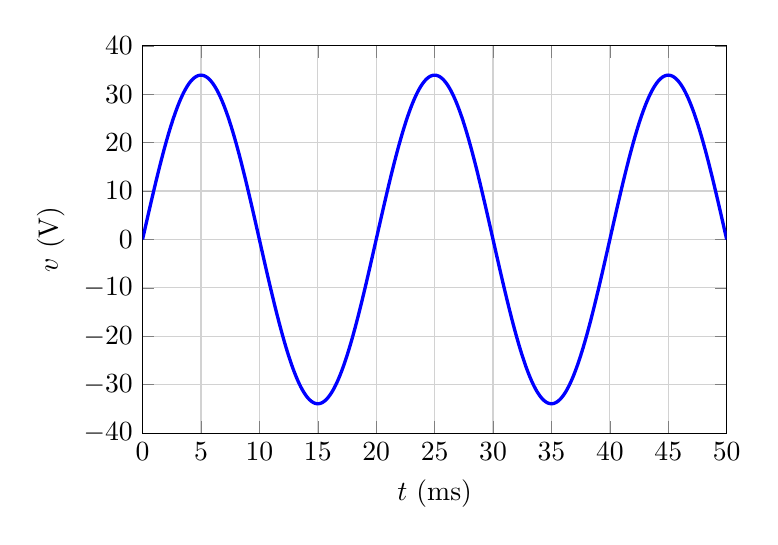
\begin{tikzpicture}
\begin{axis}[width=9cm,height=6.5cm,xmin=0,xmax=50,ymin=-40,ymax=40,
  xtick={0,5,...,50},ytick={-40,-30,...,40},grid=major,grid style={gray!35},
  xlabel={$t$ (ms)},ylabel={$v$ (V)},samples=400,domain=0:50]
\addplot[very thick,blue] {33.94*sin(18*x)};
\end{axis}
\end{tikzpicture}
\caption{Waveform (Time 5\,ms/div, Volt 10\,V/div).}
\end{figure}

\section{Discussion and answers to questions}
\begin{enumerate}[leftmargin=*]
\item \textbf{Question?} Answer.
\end{enumerate}

\section{Conclusion}
...

\end{document}
